\chapter{DFT} 

\begin{figure}[h]
    \centering
    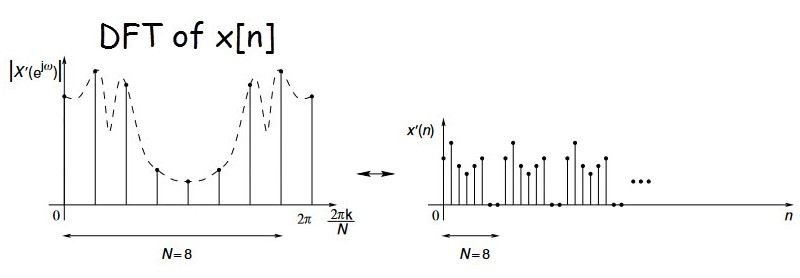
\includegraphics[scale = 0.7]{DFT.jpg}
\end{figure}  

\newpage 

\section{Introduzione alla trasformata discreta di Fuorier (DFT)}

La trasformata discreta di Fourier, comunemente nota in letteratura con l'acronimo DFT (Discrete Fourier Transform) 
risponde all'esigenza di implementare al calcolatore la trasformata di Fourier di una funzione del tempo. \newline 

Si considerino la funzione h(t) e la sua trasformata di Fourier H(f) in figura: 

\begin{figure}[h]
    \centering
    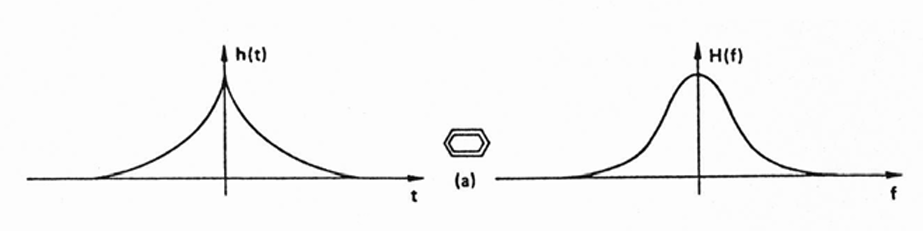
\includegraphics[scale = 0.7]{h(t) e H(f).PNG}
\end{figure} 

Per determinare la trasformata di Fourier di h(t) mediante tecniche di analisi digitale, 
è necessario campionare la funzione h(t). \newline 

Il campionamento è relaizzato moltiplicando h(t) per la sequenza campionante $\Delta_o (t)$. \newline 

Quindi, sapendo che $\Delta_o (t)$ è la seguente: 

\begin{figure}[h]
    \centering
    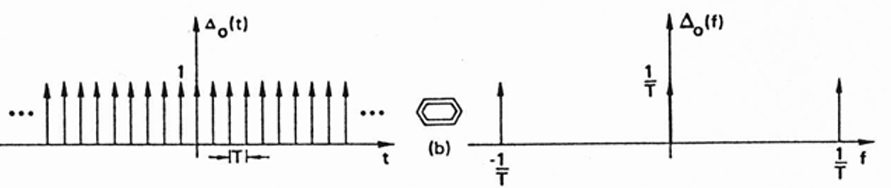
\includegraphics[scale = 0.7]{Treno di impulsi Delta_o (t).PNG}
\end{figure} 

$h(t) \cdot \Delta_o (t)$ sarà: 


\begin{figure}[h]
    \centering
    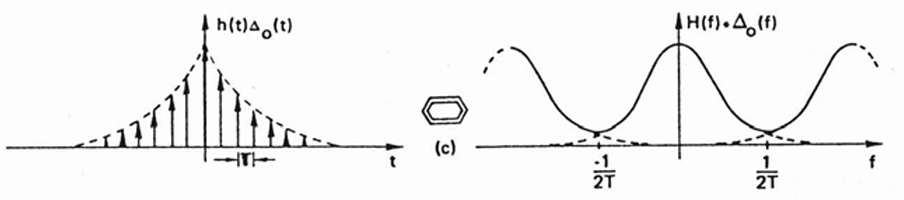
\includegraphics[scale = 0.7]{h(t) moltiplicata per il treno di impulsi.PNG}
\end{figure} 

Analizzando la figura, notiamo che la sequenza è costituita da una sequenza di implusi matematici (Delta di Dirac) 
distanziati di T l'uno dall'altro. \newline 

Il risultato del campionamento è, in Fourier, il segnale originale replicato infinte volte, centrato su un multiplo della frequenza di campionamento $\frac{1}{T}$. \newline 

Se la frequenza non è sufficientemente grande, compare il fenomeno dell'aliasing, per cui tali repliche risultano sovrapposte. \newline 

Procedendo coi passaggi, avremo che: 

\begin{figure}[h]
    \centering
    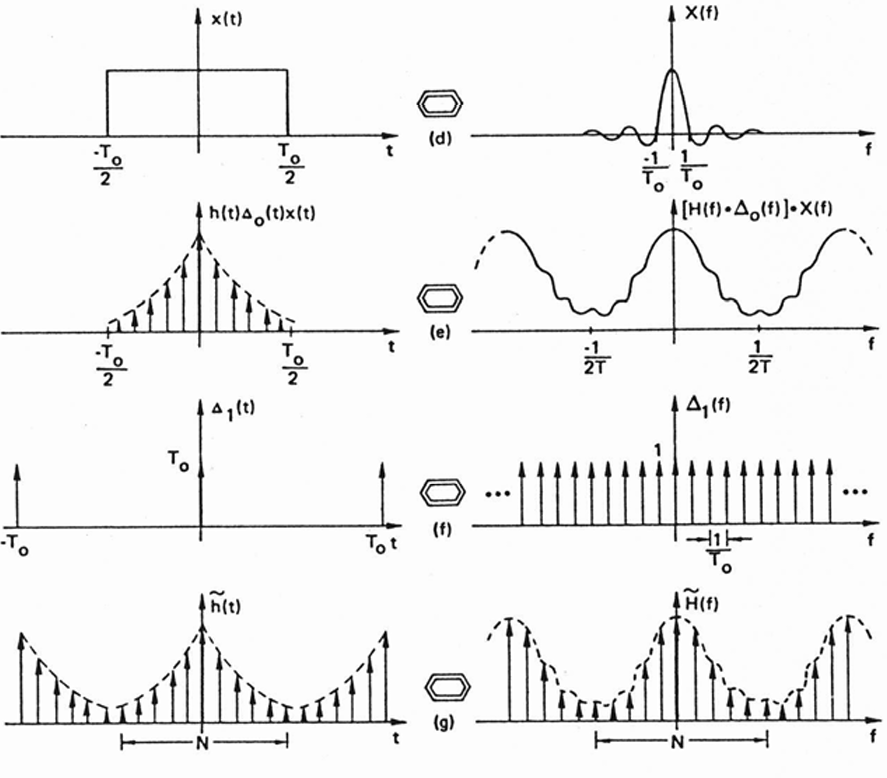
\includegraphics[scale = 0.7]{Altri passaggi per la DFT.PNG}
\end{figure} 

\newpage 

Come notiamo dalla figura, il campionamento nel dominio del tempo ha prodotto una funzione periodica in frequenza, 
mentre il campionamento nel dominio della frequenza ha prodotto una funzione periodica nel tempo. \newline 

Ciascun periodo, nel tempo e in frequenza, contiene N campioni. \newline 

\newpage 

Invece, analizzando un altro esempio di segnale, l'esponenziale bilaterale unilatera, e che quindi si sviluppa solo in $t \geq 0$ 
e ponendo la finestra di campionamento non centrata nell'origine, notiamo che: 

\begin{figure}[h]
    \centering
    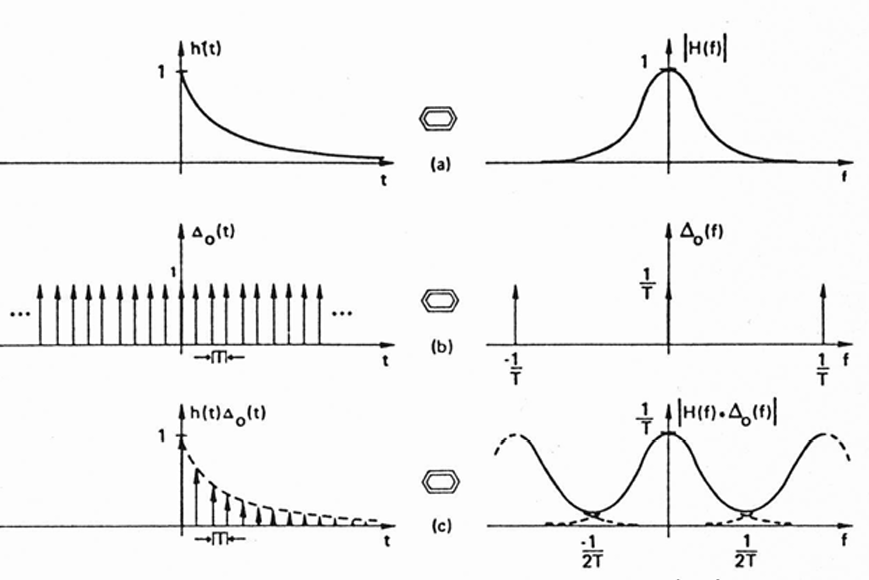
\includegraphics[scale = 0.7]{Campionamento segnale espnenzianziale unilatera.PNG}
\end{figure} 

\newpage

Formalizzando le figure in formule matematiche, notiamo che: 

{
    \Large 
    \begin{equation}
        \begin{split}
            h(t) \Delta_o (t) 
            &= 
            h(t) 
            \sum_{k = - \infty}^{\infty} 
            \delta (t - kT) 
            \\ 
            &= 
            \sum_{k = - \infty}^{\infty}
            h(kT) 
            \delta (t - kT)
        \end{split}
    \end{equation}
}

Assumendo N campioni, signfica moltiplicare la funzione precedente per x(t). \newline 

Utilizzando le figure: 

\begin{figure}[h]
    \centering
    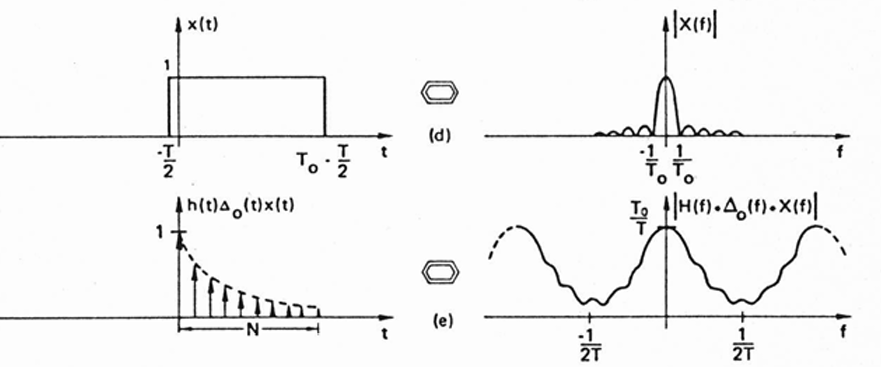
\includegraphics[scale = 0.7]{Campionamento segnale espnenzianziale unilatera step 2.PNG}
\end{figure} 

Formalizzando: 

{
    \Large 
    \begin{equation}
        \begin{split}
            h(t) \Delta_o (t) x(t) 
            &= 
            [ h(t) \sum_{k = -\infty}^{\infty} \delta (t - kT) ] x(t) 
            \\ 
            &= 
            \sum_{k = 0}^{N-1} 
            h(kT) \delta (t - kT)   
        \end{split}
    \end{equation}
}

Alla funzione campionante nel domnio della frequenza, $\Delta_l (f)$, corrispondente nel dominio del tempo: 

\begin{figure}[h]
    \centering
    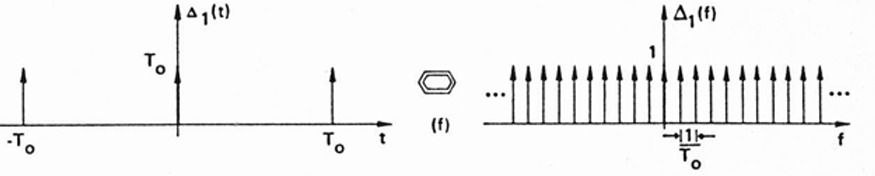
\includegraphics[scale = 0.7]{Delta_l (f).PNG}
\end{figure} 

{
    \Large 
    \begin{equation}
        \Delta_l (t) = T_o \sum_{r = -\infty}^{\infty} \delta (t - rT_o)
    \end{equation}
}

Facendo la convoluzione, notiamo che: 

\begin{figure}[h]
    \centering
    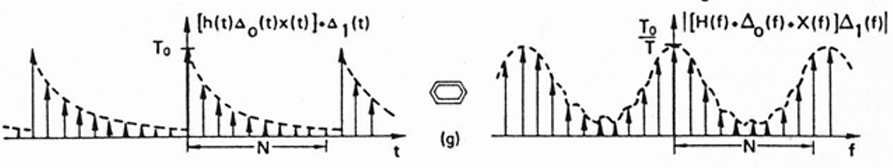
\includegraphics[scale = 0.7]{Convoluzione esponenziale DFT.PNG}
\end{figure} 

{
    \Large 
    \begin{equation}
        \begin{split}
            h^{\sim} (t) 
            &= 
            [h (t) \Delta_o (t) x(t)] * \Delta_l (t) 
            \\ 
            &= 
            [\sum_{k = 0}^{N-1} h(kT) \delta(t - kT)] 
            * 
            [T_o \sum_{r = -\infty}^{\infty} \delta (t-rT_o)]
            \\ 
            &= 
            T_o \sum_{r = \infty}^{\infty} [\sum_{k = 0}^{N-1} h(kT) \delta (t - kT -rT_o)]    
        \end{split}
    \end{equation}
}

\newpage 

\section{Casi di pratico interesse interesse}

Rispetto all'aspetto analitico, si prediligerà l'aspetto grafico nel tema della DFT. \newline 

\newpage

\subsection{Forme d'onda periodiche a banda limitata: finestra di campionamento uguale al periodo}

\begin{figure}[h]
    \centering
    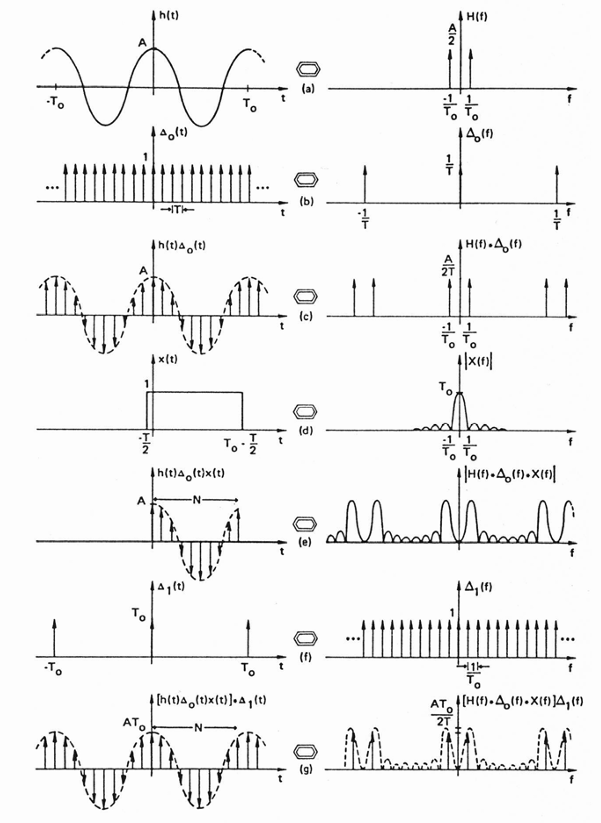
\includegraphics[scale = 0.8]{Forma d'onda periodica a banda limitata finestra di campionamento uguale al periodo.PNG}
\end{figure} 

Scorrendo rapidamente le varie parti per produrre la DFT, notiamo che: 

\begin{itemize}
    \item il campionamento nel dominio del tempo non produce aliasing 
    \item il campionamento nel dominio del tempo produce una scalatura delle ampiezze nel dominio delle frequenze, per cui l'area originale (A/2) della Delta di Dirac viene ridotta di un fattore 1/T, quindi diventa A/2T 
    \item la finestra di campionamento include esattamente un periodo della funzione cosinusoidale, e gli N campioni nel dominio del tempo sono contenuti entro questo periodo 
    \item il risultato del prodotto nel dominio del tempo fra la forma d'onda campionata e la finestra di campionamento ha uno spettro fortemente distorto rispetto alla H(f) originale 
    \item quando, però, si effettua il campionamento nel dominio della frequenza, questa distorsione sparisce
\end{itemize}

\newpage 

\subsection{Forme d'onda periodiche a banda limitata: finestra di campionamento diversa dal periodo}